
%% Energy Questions used on the
%% NYSED Physics Regents Examination
%%--------------------------------------------------

%% this section contains 42 problems


%% Section June2015
%%--------------------
\element{nysed}{
\begin{question}{June2015-Q15}
    A block slides across a rough, horizontal tabletop.
    As the block comes to rest,
        there is an increase in the block-tabletop system's:
    \begin{choices}
        \wrongchoice{gravitational potential energy}
        \wrongchoice{kinetic energy}
        \wrongchoice{elastic potential energy}
      \correctchoice{internal (thermal) energy}
    \end{choices}
\end{question}
}

\element{nysed}{
\begin{question}{June2015-Q45}
    A compressed spring in a toy is used to launch a \SI{5.00}{\gram} ball. 
    If the ball leaves the toy with an initial horizontal speed of \SI{5.00}{\meter\per\second},
        the minimum amount of potential energy stored in the compressed spring was:
    \begin{multicols}{2}
    \begin{choices}
        \wrongchoice{\SI{0.0125}{\joule}}
        \wrongchoice{\SI{0.0250}{\joule}}
      \correctchoice{\SI{0.0625}{\joule}}
        \wrongchoice{\SI{0.125}{\joule}}
    \end{choices}
    \end{multicols}
\end{question}
}


%% Section June2014
%%--------------------
\element{nysed}{
\begin{question}{June2014-Q31}
    A shopping cart slows as it moves along a level floor.
    Which statement describes the energies of the cart?
    \begin{choices}
      \correctchoice{the kinetic energy decreases and the gravitational potential energy decreases}
        \wrongchoice{the kinetic energy increases and the gravitational potential energy remains the same}
        \wrongchoice{the kinetic energy increases and the gravitational potential energy decreases}
        \wrongchoice{the kinetic energy decreases and the gravitational potential energy remains the same}
    \end{choices}
\end{question}
}

\element{nysed}{
\begin{question}{June2014-Q42}
    A \SI{25}{\gram} paper cup falls from rest off the edge of a tabletop \SI{0.90}{\meter} above the floor.
    If the cup has \SI{0.20}{\joule} of kinetic energy when it hits the floor,
        what is the total amount of energy converted into internal thermal energy during the cups fall?
    \begin{multicols}{2}
    \begin{choices}
      \correctchoice{\SI{0.02}{\joule}}
        \wrongchoice{\SI{2.2}{\joule}}
        \wrongchoice{\SI{0.22}{\joule}}
        \wrongchoice{\SI{2.20}{\joule}}
    \end{choices}
    \end{multicols}
\end{question}
}

\element{nysed}{
\begin{question}{June2014-Q44}
    Which graph best represents an object in equilibrium moving in a straight line?
    \begin{multicols}{2}
    \begin{choices}
        \AMCboxDimensions{down=-2.5em}
        \correctchoice{
            \begin{tikzpicture}
                \begin{axis}[
                    axis y line=left,
                    axis x line=bottom,
                    axis line style={->},
                    xlabel={time},
                    xtick=\empty,
                    ylabel={kinetic energy},
                    ytick=\empty,
                    xmin=0,xmax=11,
                    ymin=0,ymax=11,
                    width=\columnwidth,
                ]
                \addplot[line width=1pt,domain=0:10]{8};
                \end{axis}
            \end{tikzpicture}
        }
        \wrongchoice{
            \begin{tikzpicture}
                \begin{axis}[
                    axis y line=left,
                    axis x line=bottom,
                    axis line style={->},
                    xlabel={time},
                    xtick=\empty,
                    ylabel={distance},
                    ytick=\empty,
                    xmin=0,xmax=11,
                    ymin=0,ymax=11,
                    width=\columnwidth,
                ]
                \addplot[line width=1pt,domain=0:10]{0.1*x*x};
                \end{axis}
            \end{tikzpicture}
        }
        \wrongchoice{
            \begin{tikzpicture}
                \begin{axis}[
                    axis y line=left,
                    axis x line=bottom,
                    axis line style={->},
                    xlabel={time},
                    xtick=\empty,
                    ylabel={momentum},
                    ytick=\empty,
                    xmin=0,xmax=11,
                    ymin=0,ymax=11,
                    width=\columnwidth,
                ]
                \addplot[line width=1pt,domain=0:10]{x};
                \end{axis}
            \end{tikzpicture}
        }
        \wrongchoice{
            \begin{tikzpicture}
                \begin{axis}[
                    axis y line=left,
                    axis x line=bottom,
                    axis line style={->},
                    xlabel={time},
                    xtick=\empty,
                    ylabel={velocity},
                    ytick=\empty,
                    xmin=0,xmax=11,
                    ymin=0,ymax=11,
                    width=\columnwidth,
                ]
                \addplot[line width=1pt,domain=0:10]{10-x};
                \end{axis}
            \end{tikzpicture}
        }
    \end{choices}
    \end{multicols}
\end{question}
}

%% Section June2013
%%--------------------
\element{nysed}{
\begin{question}{June2013-Q21}
    In the diagram below, an ideal pendulum released from position
        $A$ swings freely to position $B$.
    \begin{center}
    \begin{tikzpicture}
        %% Ceiling
        \draw[thick] (-2,0) -- (2,0);
        \node[anchor=south,pattern=north east lines,minimum width=4cm] at (0,0) {};
        %% Pendulum
        \draw (0,0) -- (250:3cm);
        \draw[fill] (250:3cm) circle (3pt)
            node[below=1ex] {$A$};
        \draw (0,0) -- (290:3cm);
        \draw[fill] (290:3cm) circle (3pt)
            node[below=1ex] {$B$};
        \draw[dotted,->] (250:3cm) arc (250:270:3cm);
        \draw[dotted] (270:3cm) arc (270:290:3cm);
    \end{tikzpicture}
    \end{center}
    As the pendulum swings from $A$ to $B$, its total mechanical energy
    \begin{choices}
        \wrongchoice{decreases, then increases}
        \wrongchoice{increases, only}
        \wrongchoice{increases, then decreases}
      \correctchoice{remains the same}
    \end{choices}
\end{question}
}

\element{nysed}{
\begin{question}{June2013-Q45}
    Which graph best represents the relationship between the kinetic energy
        and the speed of a freely falling object?
    \begin{multicols}{2}
    \begin{choices}
        \AMCboxDimensions{down=-2.0em}
        \correctchoice{
            \begin{tikzpicture}
                \begin{axis}[
                    axis y line=left,
                    axis x line=bottom,
                    axis line style={->},
                    xlabel={speed},
                    xtick=\empty,
                    ylabel={kinetic energy},
                    ytick=\empty,
                    xmin=0,xmax=11,
                    ymin=0,ymax=11,
                    width=\columnwidth,
                    very thin,
                ]
                \addplot[line width=1pt,domain=0:10]{0.1*x*x};
                \end{axis}
            \end{tikzpicture}
        }
        \wrongchoice{
            \begin{tikzpicture}
                \begin{axis}[
                    axis y line=left,
                    axis x line=bottom,
                    axis line style={->},
                    xlabel={speed},
                    xtick=\empty,
                    ylabel={kinetic energy},
                    ytick=\empty,
                    xmin=0,xmax=11,
                    ymin=0,ymax=11,
                    width=\columnwidth,
                    very thin,
                ]
                \addplot[line width=1pt,domain=0:10]{x};
                \end{axis}
            \end{tikzpicture}
        }
        \wrongchoice{
            \begin{tikzpicture}
                \begin{axis}[
                    axis y line=left,
                    axis x line=bottom,
                    axis line style={->},
                    xlabel={speed},
                    xtick=\empty,
                    ylabel={kinetic energy},
                    ytick=\empty,
                    xmin=0,xmax=11,
                    ymin=0,ymax=11,
                    width=\columnwidth,
                    very thin,
                ]
                \addplot[line width=1pt,domain=0:10]{10-x};
                \end{axis}
            \end{tikzpicture}
        }
        \wrongchoice{
            \begin{tikzpicture}
                \begin{axis}[
                    axis y line=left,
                    axis x line=bottom,
                    axis line style={->},
                    xlabel={speed},
                    xtick=\empty,
                    ylabel={kinetic energy},
                    ytick=\empty,
                    xmin=0,xmax=11,
                    ymin=0,ymax=11,
                    width=\columnwidth,
                    very thin,
                ]
                \addplot[line width=1pt,domain=0:10]{5/x};
                \end{axis}
            \end{tikzpicture}
        }
    \end{choices}
    \end{multicols}
\end{question}
}


%% Section June2012
%%--------------------
\element{nysed}{
\begin{question}{June2012-Q14}
    A car uses its brakes to stop on a level road.
    During this process, there must be a conversion of kinetic energy into:
    \begin{choices}
        \wrongchoice{light energy}
        \wrongchoice{nuclear energy}
        \wrongchoice{gravitational potential energy}
      \correctchoice{internal energy}
    \end{choices}
\end{question}
}

\element{nysed}{
\begin{question}{June2012-Q50}
    A pendulum is made from a \SI{7.50}{\kilo\gram} mass attached to a rope connected to the ceiling of a gymnasium.
    The mass is pushed to the side until its position $A$,
        \SI{1.5}{\meter} higher than its equilibrium position.
    After it is released from rest at position $A$, the pendulum moved freely back and forth between positions $A$ and $B$,
        as shown in the diagram below.
    \begin{center}
    \begin{tikzpicture}
        %% Ceiling
        \draw (-2,0) -- (2,0);
        \node[anchor=south,fill,pattern=north east lines,minimum width=4cm] at (0,0) {};
        \node[anchor=south] at (0,1em) {Ceiling};
        %% height
        \draw[dashed] (-3,-4.33) -- (3,-4.33);
        \draw[dashed] (-3,-5) -- (3,-5);
        \draw[<->] (1,-4.33) -- (1,-5) node[pos=0.5,anchor=west] {\SI{1.5}{\meter}};
        %% pendulums
        \draw[dashed] (0,0) -- (240:5);
        \draw[thick] (0,0) -- (270:5);
        %% options
        \foreach \x/\y in {240/A,300/B}
            \draw[fill=white!90!black] (\x:5) circle (5pt) node[anchor=north west] {$\y$};
        \draw[fill=white!90!black] (270:5) circle (5pt) node[anchor=north,yshift=-5pt,text width=5em,text centered] {Equilibrium Position};
        \node[pin={120:\SI{7.5}{\kilo\gram}}] at (240:5) {};
    \end{tikzpicture}
    \end{center}
    What is the total amount of kinetic energy that the mass has as it swings freely through its equilibrium position?
    \begin{multicols}{2}
    \begin{choices}
        \wrongchoice{\SI{11}{\joule}}
        \wrongchoice{\SI{94}{\joule}}
      \correctchoice{\SI{110}{\joule}}
        \wrongchoice{\SI{920}{\joule}}
    \end{choices}
    \end{multicols}
\end{question}
}


%% Section June2011
%%--------------------
\element{nysed}{
\begin{question}{June2011-Q09}
    As a box pushes \SI{30}{\meter} across a horizontal floor by a constant horizontal force of \SI{25}{\newton},
        the kinetic energy of the box increases by \SI{300}{\joule}.
    How much total internal energy is produced during this process?
    \begin{multicols}{2}
    \begin{choices}
        \wrongchoice{\SI{150}{\joule}}
        \wrongchoice{\SI{250}{\joule}}
      \correctchoice{\SI{450}{\joule}}
        \wrongchoice{\SI{750}{\joule}}
    \end{choices}
    \end{multicols}
\end{question}
}

\element{nysed}{
\begin{question}{June2011-Q14}
    Which statement describes the kinetic energy and total mechanical energy of a block as it is pulled at constant speed up an incline?
    \begin{choices}
        \wrongchoice{Kinetic energy decreases and total mechanical energy increases}
        \wrongchoice{Kinetic energy decreases and total mechanical energy remains the same}
      \correctchoice{Kinetic energy remains the same and total mechanical energy increases}
        \wrongchoice{Kinetic energy remains the same and total mechanical energy remains the same}
    \end{choices}
\end{question}
}


%% Section June2010
%%--------------------
\element{nysed}{
\begin{question}{June2010-Q15}
    A wound spring provides the energy to propel a toy car across a level floor.
    At time $t_1$, the car is moving at speed $v_1$ across the floor and the spring is unwinding, as shown below.
    At time $t_f$, the spring has fully unwound and the car has coasted to a stop.
    \begin{center}
        %% NOTE: keep
        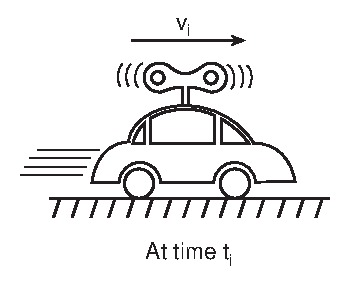
\includegraphics[keepaspectratio,scale=0.55]{June2010-Q15-left}
        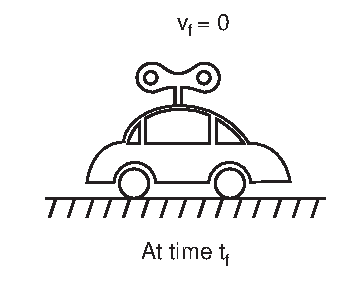
\includegraphics[keepaspectratio,scale=0.55]{June2010-Q15-right}
    \end{center}
    Which statement best describes the transformation of energy that occurs between times $t_1$ and $t_f$?
    \begin{choices}
        \wrongchoice{Gravitational potential energy at $t_1$ is converted to internal energy at $t_f$.}
        \wrongchoice{Elastic potential energy at $t_1$ is converted to kinetic energy at $t_f$.}
      \correctchoice{Both elastic potential energy and kinetic energy at $t_1$ are converted to internal energy at $t_f$.}
        \wrongchoice{Both kinetic energy and internal energy at $t_1$ are converted to elastic potential energy at $t_f$.}
    \end{choices}
\end{question}
}

\element{nysed}{
\begin{question}{June2010-Q39}
    A ball is dropped from the top of a cliff.
    Which graph best represents the relationship between the ball's total energy and elapsed time as the ball falls to the ground?
    [Neglect friction.]
    \begin{multicols}{2}
    \begin{choices}
        \AMCboxDimensions{down=-2.5em}
        \correctchoice{
            \begin{tikzpicture}
                \begin{axis}[
                    axis y line=left,
                    axis x line=bottom,
                    axis line style={->},
                    xlabel={time},
                    xtick=\empty,
                    ylabel={total energy},
                    ytick=\empty,
                    xmin=0,xmax=11,
                    ymin=0,ymax=11,
                    width=\columnwidth,
                    very thin,
                ]
                \addplot[line width=1pt,domain=0:10]{8};
                \end{axis}
            \end{tikzpicture}
        }
        \wrongchoice{
            \begin{tikzpicture}
                \begin{axis}[
                    axis y line=left,
                    axis x line=bottom,
                    axis line style={->},
                    xlabel={time},
                    xtick=\empty,
                    ylabel={total energy},
                    ytick=\empty,
                    xmin=0,xmax=11,
                    ymin=0,ymax=11,
                    width=\columnwidth,
                    very thin,
                ]
                \addplot[line width=1pt,domain=0:10]{x};
                \end{axis}
            \end{tikzpicture}
        }
        \wrongchoice{
            \begin{tikzpicture}
                \begin{axis}[
                    axis y line=left,
                    axis x line=bottom,
                    axis line style={->},
                    xlabel={time},
                    xtick=\empty,
                    ylabel={total energy},
                    ytick=\empty,
                    xmin=0,xmax=11,
                    ymin=0,ymax=11,
                    width=\columnwidth,
                    very thin,
                ]
                \addplot[line width=1pt,domain=0:10]{0.1*x*x};
                \end{axis}
            \end{tikzpicture}
        }
        \wrongchoice{
            \begin{tikzpicture}
                \begin{axis}[
                    axis y line=left,
                    axis x line=bottom,
                    axis line style={->},
                    xlabel={time},
                    xtick=\empty,
                    ylabel={total energy},
                    ytick=\empty,
                    xmin=0,xmax=11,
                    ymin=0,ymax=11,
                    width=\columnwidth,
                    very thin,
                ]
                \addplot[line width=1pt,domain=0:10]{10-x};
                \end{axis}
            \end{tikzpicture}
        }
    \end{choices}
    \end{multicols}
\end{question}
}

\element{nysed}{
\begin{question}{June2010-Q40}
    A child, starting from rest at the top of a playground slide,
        reaches a speed of \SI{7.0}{\meter\per\second} at the bottom of the slide.
    What is the vertical height of the slide?
    [Neglect friction.]
    \begin{multicols}{2}
    \begin{choices}
        \wrongchoice{\SI{0.71}{\meter}}
        \wrongchoice{\SI{1.4}{\meter}}
      \correctchoice{\SI{2.5}{\meter}}
        \wrongchoice{\SI{3.5}{\meter}}
    \end{choices}
    \end{multicols}
\end{question}
}


%% Section June2009
%%--------------------
\element{nysed}{
\begin{question}{June2009-Q15}
    As a ball falls freely toward the ground,
        its total mechanical energy:
    \begin{choices}
        \wrongchoice{decreases}
        \wrongchoice{increases}
      \correctchoice{remains the same}
    \end{choices}
\end{question}
}


%% Section Jan2009
%%--------------------
\element{nysed}{
\begin{question}{Jan2009-Q39}
    A wooden crate is pushed at constant speed across a level wooden floor.
    Which graph best represents the relationship between the total mechanical energy of the crate and the duration of time the crate is pushed?
    \begin{multicols}{2}
    \begin{choices}
        \AMCboxDimensions{down=-2.5em}
        \correctchoice{
            \begin{tikzpicture}
                \begin{axis}[
                    axis y line=left,
                    axis x line=bottom,
                    axis line style={->},
                    xlabel={time},
                    xtick=\empty,
                    ylabel={total energy},
                    ytick=\empty,
                    xmin=0,xmax=11,
                    ymin=0,ymax=11,
                    width=\columnwidth,
                    very thin,
                ]
                \addplot[line width=1pt,domain=0:10]{8};
                \end{axis}
            \end{tikzpicture}
        }
        \wrongchoice{
            \begin{tikzpicture}
                \begin{axis}[
                    axis y line=left,
                    axis x line=bottom,
                    axis line style={->},
                    xlabel={time},
                    xtick=\empty,
                    ylabel={total energy},
                    ytick=\empty,
                    xmin=0,xmax=11,
                    ymin=0,ymax=11,
                    width=\columnwidth,
                    very thin,
                ]
                \addplot[line width=1pt,domain=0:10]{0.1*x*x};
                \end{axis}
            \end{tikzpicture}
        }
        \wrongchoice{
            \begin{tikzpicture}
                \begin{axis}[
                    axis y line=left,
                    axis x line=bottom,
                    axis line style={->},
                    xlabel={time},
                    xtick=\empty,
                    ylabel={total energy},
                    ytick=\empty,
                    xmin=0,xmax=11,
                    ymin=0,ymax=11,
                    width=\columnwidth,
                    very thin,
                ]
                \addplot[line width=1pt,domain=0:10]{x};
                \end{axis}
            \end{tikzpicture}
        }
        \wrongchoice{
            \begin{tikzpicture}
                \begin{axis}[
                    axis y line=left,
                    axis x line=bottom,
                    axis line style={->},
                    xlabel={time},
                    xtick=\empty,
                    ylabel={total energy},
                    ytick=\empty,
                    xmin=0,xmax=11,
                    ymin=0,ymax=11,
                    width=\columnwidth,
                    very thin,
                ]
                \addplot[line width=1pt,domain=0:10]{10 - 0.1*(x-10)*(x-10)};
                \end{axis}
            \end{tikzpicture}
        }
    \end{choices}
    \end{multicols}
\end{question}
}

\element{nysed}{
\begin{question}{Jan2009-Q41}
    A book of mass $m$ falls freely from rest to the floor from the top of a desk of height $h$.
    what is the speed of the book upon striking the floor?
    \begin{multicols}{2}
    \begin{choices}
      \correctchoice{$\sqrt{2gh}$}
        \wrongchoice{$2gh$}
        \wrongchoice{$mgh$}
        \wrongchoice{$mh$}
    \end{choices}
    \end{multicols}
\end{question}
}


%% Section June2008
%%--------------------
\element{nysed}{
\begin{question}{June2008-Q18}
    A car travels at constant speed $v$ up a hill from point $A$ to point $B$, as shown in the diagram below.
    \begin{center}
    \begin{tikzpicture}
        %% Ground
        \draw (0,0) -- (6,0);
        \node[anchor=north,fill,pattern=north east lines,minimum width=6cm] at (3,0) {};
        \node[anchor=north] at (3,-1em) {Horizontal};
        \draw (0,0) -- (15:{6/cos(15)});
        %% points A and B
        \fill (15:1) circle (1.5pt) node[anchor=south] {$A$};
        \fill (15:6) circle (1.5pt) node[anchor=south] {$B$};
        %% car
        \path (15:3) ++(110:0.2)  node[draw,minimum height=0.5cm,minimum width=1.5cm,anchor=south,rotate=15] (C) {};
        \draw[fill=white] (C.south west) ++(15:0.4) circle (0.2);
        \draw[fill=black] (C.south west) ++(15:0.4) circle (1pt);
        \draw[fill=white] (C.south east) ++(195:0.4) circle (0.2);
        \draw[fill=black] (C.south east) ++(195:0.4) circle (1pt);
        %% velocity
        \draw[thick,->] (C.east) -- ++(15:1) node[pos=0.5,anchor=south,rotate=15] {$v$};
    \end{tikzpicture}
    \end{center}
    As the car travels from $A$ to $B$, its gravitational potential energy:
    \begin{choices}
        \wrongchoice{increases and its kinetic energy decreases}
      \correctchoice{increases and its kinetic energy remains the same}
        \wrongchoice{remains the same and its kinetic energy decreases}
        \wrongchoice{remains the same and its kinetic remains the same}
    \end{choices}
\end{question}
}

\element{nysed}{
\begin{question}{June2008-Q45}
    An object is thrown vertically upward, which pair of graphs best represents the object's kinetic energy and gravitational potential energy as functions of its displacement while it rises?
    \begin{choices}
        \AMCboxDimensions{down=-2.5em}
        \correctchoice{
            \begin{tikzpicture}
                \begin{groupplot}[
                        axis y line=left,
                        axis x line=bottom,
                        axis line style={->},
                        group style={group size=2 by 1},
                        xlabel={displacement},
                        xtick=\empty,
                        ytick=\empty,
                        xmin=0,xmax=11,
                        ymin=0,ymax=11,
                        width=0.5\columnwidth,
                    ]
                    \nextgroupplot[
                        ylabel={kinetic energy},
                    ] \addplot[line width=1pt,domain=0:10] {10-x};
                    \nextgroupplot[
                        ylabel={potential energy},
                    ] \addplot[line width=1pt,domain=0:10] {x};
                \end{groupplot}
            \end{tikzpicture}
        }
        \wrongchoice{
            \begin{tikzpicture}
                \begin{groupplot}[
                        axis y line=left,
                        axis x line=bottom,
                        axis line style={->},
                        group style={group size=2 by 1},
                        xlabel={displacement},
                        xtick=\empty,
                        ytick=\empty,
                        xmin=0,xmax=11,
                        ymin=0,ymax=11,
                        width=0.5\columnwidth,
                    ]
                    \nextgroupplot[
                        ylabel={kinetic energy},
                    ] \addplot[line width=1pt,domain=0:10] {x};
                    \nextgroupplot[
                        ylabel={potential energy},
                    ] \addplot[line width=1pt,domain=0:10] {x};
                \end{groupplot}
            \end{tikzpicture}
        }
        \wrongchoice{
            \begin{tikzpicture}
                \begin{groupplot}[
                        axis y line=left,
                        axis x line=bottom,
                        axis line style={->},
                        group style={group size=2 by 1},
                        xlabel={displacement},
                        xtick=\empty,
                        ytick=\empty,
                        xmin=0,xmax=11,
                        ymin=0,ymax=11,
                        width=0.5\columnwidth,
                    ]
                    \nextgroupplot[
                        ylabel={kinetic energy},
                    ] \addplot[line width=1pt,domain=0:10] {8};
                    \nextgroupplot[
                        ylabel={potential energy},
                    ] \addplot[line width=1pt,domain=0:10] {10-x};
                \end{groupplot}
            \end{tikzpicture}
        }
        \wrongchoice{
            \begin{tikzpicture}
                \begin{groupplot}[
                        axis y line=left,
                        axis x line=bottom,
                        axis line style={->},
                        group style={group size=2 by 1},
                        xlabel={displacement},
                        xtick=\empty,
                        ytick=\empty,
                        xmin=0,xmax=11,
                        ymin=0,ymax=11,
                        width=0.5\columnwidth,
                    ]
                    \nextgroupplot[
                        ylabel={kinetic energy},
                    ] \addplot[line width=1pt,domain=0:10] {10-x};
                    \nextgroupplot[
                        ylabel={potential energy},
                    ] \addplot[line width=1pt,domain=0:10] {8};
                \end{groupplot}
            \end{tikzpicture}
        }
    \end{choices}
\end{question}
}


%% Section Jan2008
%%--------------------
\element{nysed}{
\begin{question}{Jan2008-Q42}
    A car with mass $m$ possesses momentum of magnitude $p$.
    Which expression correctly represents the kinetic energy, $KE$,
        of the car in terms of $m$ and $p$?
    \begin{multicols}{2}
    \begin{choices}
        \wrongchoice{$KE = \dfrac{p}{2m}$}
        \wrongchoice{$KE = \dfrac{mp^2}{2}$}
        \wrongchoice{$KE = \dfrac{mp}{2}$}
      \correctchoice{$KE = \dfrac{p^2}{2m}$}
    \end{choices}
    \end{multicols}
\end{question}
}


%% Section June2007
%%--------------------
\element{nysed}{
\begin{question}{June2007-Q12}
    A horizontal force of \SI{5.0}{\newton} acts on a \SI{3.0}{\kilo\gram} mass over a distance of \SI{6.0}{\meter} along a horizontal,
        frictionless surface.
    What is the change in kinetic energy of the mass during its movement over the \SI{6.0}{\meter} distance?
    \begin{multicols}{2}
    \begin{choices}
      \correctchoice{\SI{30}{\joule}}
        \wrongchoice{\SI{90}{\joule}}
        \wrongchoice{\SI{6.0}{\joule}}
        \wrongchoice{\SI{15}{\joule}}
    \end{choices}
    \end{multicols}
\end{question}
}


%% Section Jan2007
%%--------------------
\element{nysed}{
\begin{question}{Jan2007-Q44}
    A \SI{1.00}{\kilo\gram} ball is dropped from the top of a building.
    Just before striking the ground, the ball's speed is \SI{12.0}{\meter\per\second}.
    What was the ball's gravitational potential energy,
        relative to the ground, at the instant it was dropped?
    [Neglect friction.]
    \begin{multicols}{2}
    \begin{choices}
      \correctchoice{\SI{72.0}{\joule}}
        \wrongchoice{\SI{144}{\joule}}
        \wrongchoice{\SI{6.00}{\joule}}
        \wrongchoice{\SI{24.0}{\joule}}
    \end{choices}
    \end{multicols}
\end{question}
}


%% Section June2006
%%--------------------
\element{nysed}{
\begin{question}{June2006-Q14}
    The potential energy storied in a compressed spring is to the change in the spring's length as the kinetic energy of a moving body is to the body's
    \begin{multicols}{2}
    \begin{choices}
      \correctchoice{speed}
        \wrongchoice{mass}
        \wrongchoice{radius}
        \wrongchoice{acceleration}
    \end{choices}
    \end{multicols}
\end{question}
}

\element{nysed}{
\begin{question}{June2006-Q15}
    The diagram below shows an ideal simple pendulum.
    \begin{center}
    \begin{tikzpicture}
        \draw (-2,0) -- (2,0);
        \node[anchor=south,fill,pattern=north east lines,minimum width=4cm, minimum height=0.05cm] at (0,0) {};
        %\foreach \x in {-20,-18,...,20}
        %    \draw[thin] (\x mm,0) -- ++ (40:0.15cm);
        %% Pendulums
        %\node[fill=white,draw,circle,minimum size=8pt] (B) at (240:3cm) {};
        \node[fill=white,draw,circle,fill=white!90!black,minimum size=8pt] (B) at (225:3cm) {};
        \node[fill=white,draw,circle,fill=white!90!black,minimum size=8pt] (A) at (270:3cm) {};
        %% Draw string
        \draw (0,0) -- (B);
        \draw (0,0) -- (A);
        \draw[thick,->] (265:3cm) arc (265:230:3cm);
        %% Labels
        \node[below=1em] at (A) {$A$};
        \node[below=1em] at (B) {$B$};
    \end{tikzpicture}
    \end{center}
    As the pendulum swings from position $A$ to position $B$,
        what happens to its total mechanical energy?
    [Neglect friction.]
    \begin{choices}
      \correctchoice{It remains the same}
        \wrongchoice{It decreases}
        \wrongchoice{It increases}
    \end{choices}
\end{question}
}


%% Section Jan2006
%%--------------------
\element{nysed}{
\begin{question}{Jan2006-Q19}
    A \SI{55.0}{\kilo\gram} diver falls freely from a diving platform that is \SI{3.00}{\meter} above the surface of the water in a pool.
    When she is \SI{1.00}{\meter} above the water,
        what are her gravitational potential energy and kinetic energy with respect to the water's surface?
    %% total energy 1617 J
    \begin{choices}
      \correctchoice{$PE=\SI{540}{\joule}$ and $KE=\SI{1080}{\joule}$}
        \wrongchoice{$PE=\SI{810}{\joule}$ and $KE=\SI{810}{\joule}$}
        \wrongchoice{$PE=\SI{1620}{\joule}$ and $KE=\SI{0}{\joule}$}
        \wrongchoice{$PE=\SI{1080}{\joule}$ and $KE=\SI{540}{\joule}$}
    \end{choices}
\end{question}
}


%% Section June2005
%%--------------------
\element{nysed}{
\begin{question}{June2005-Q39}
    When a \SI{1.53}{\kilo\gram} mass is placed on a spring with a spring constant of \SI{30.0}{\newton\per\meter},
        the spring is compressed \SI{0.500}{\meter}.
    How much energy is stored in the spring?
    \begin{multicols}{2}
    \begin{choices}
      \correctchoice{\SI{3.75}{\joule}}
        \wrongchoice{\SI{7.50}{\joule}}
        \wrongchoice{\SI{15.0}{\joule}}
        \wrongchoice{\SI{30.0}{\joule}}
    \end{choices}
    \end{multicols}
\end{question}
}


%% Section Jan2005
%%--------------------
\element{nysed}{
\begin{question}{Jan2005-Q05}
    In the diagram below, a \SI{10}{\kilo\gram} block is at rest on a plane inclined at \ang{15} to the horizontal.
    \begin{center}
    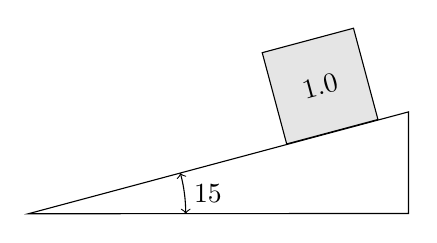
\begin{tikzpicture}
        %% 15 degree incline
        \draw (0,0) --  (15:5) -- ++(270:1.29) --cycle;
        \draw[<->] (2,0) arc (0:15:2) node[pos=0.5,anchor=west] {\ang{15}};
        %% 1.0 kg block
        \node[draw,anchor=south,minimum size=1.2cm,rotate=15,fill=white!90!black] at (15:4) {\SI{1.0}{\kilo\gram}};
    \end{tikzpicture}
    \end{center}
    As the angle of the incline is increased to \ang{30},
        the mass of the block will:
    \begin{choices}
      \correctchoice{remain the same}
        \wrongchoice{decrease}
        \wrongchoice{increase}
    \end{choices}
\end{question}
}

\element{nysed}{
\begin{question}{Jan2005-Q06}
    If the direction of a moving car changes and its speed remains constant,
        which quantity must remain the same?
    \begin{multicols}{2}
    \begin{choices}
        \wrongchoice{velocity}
        \wrongchoice{displacement}
        \wrongchoice{momentum}
      \correctchoice{kinetic energy}
    \end{choices}
    \end{multicols}
\end{question}
}

\element{nysed}{
\begin{question}{Jan2005-Q46}
    As shown in the diagram below, a \SI{0.5}{\meter} long spring is stretched from its equilibrium position to a length of \SI{1.00}{\meter} by a weight.
    \begin{center}
    \begin{tikzpicture}
        \begin{scope}[xshift=-2cm]
            %% Title
            \node[anchor=south,text centered] at (0.5,0.2cm) {Unstretched};
            %% Celiing
            \draw (-1,0) --  (2,0);
            \node[anchor=south,fill,pattern=north east lines,minimum width=3cm, minimum height=0.05cm] at (0.5,0) {};
            %% Spring
            \draw[thick,decoration={aspect=0.2,segment length=1.5mm,amplitude=4mm,coil},decorate] (0,0) -- (0,-1.5);
            \draw[dashed]  (0,-1.5) -- ++(0:1cm);
            %% Ruler
            \draw[<->] (1.5,0) -- (1.5,-1.5) node[pos=0.5,anchor=center,fill=white] {\SI{0.50}{\meter}};
        \end{scope}
        \begin{scope}[xshift=+2cm]
            %% Title
            \node[anchor=south,text centered] at (0.5,0.2cm) {Stretched};
            %% Celiing
            \draw (-1,0) --  (2,0);
            \node[anchor=south,fill,pattern=north east lines,minimum width=3cm, minimum height=0.05cm] at (0.5,0) {};
            %% Weight
            \node[anchor=north,draw,minimum size=1cm] (M) at (0,-3) {Weight};
            %% Spring
            \draw[thick,decoration={aspect=0.2,segment length=3mm,amplitude=4mm,coil},decorate] (0,0) -- (0,-3);
            \draw[dashed]  (0,-3) -- ++(0:1cm);
            %% Ruler
            \draw[<->] (1.5,0) -- (1.5,-3) node[pos=0.5,anchor=center,fill=white] {\SI{1.00}{\meter}};
        \end{scope}
    \end{tikzpicture}
    \end{center}
    If \SI{15}{\joule} of energy are stored in the stretched spring,
        what is the value of the spring constant?
    \begin{multicols}{2}
    \begin{choices}
      \correctchoice{\SI{120}{\newton\per\meter}}
        \wrongchoice{\SI{240}{\newton\per\meter}}
        \wrongchoice{\SI{30}{\newton\per\meter}}
        \wrongchoice{\SI{60}{\newton\per\meter}}
    \end{choices}
    \end{multicols}
\end{question}
}


%% Section June2004
%%--------------------
\element{nysed}{
\begin{question}{June2004-Q14}
    A \SI{5}{\newton} force causes a spring to stretch \SI{0.2}{\meter}.
    What is the potential energy stored in the stretched spring?
    \begin{multicols}{2}
    \begin{choices}
      \correctchoice{\SI{0.5}{\joule}}
        \wrongchoice{\SI{1.}{\joule}}
        \wrongchoice{\SI{0.2}{\joule}}
        \wrongchoice{\SI{0.1}{\joule}}
    \end{choices}
    \end{multicols}
\end{question}
}

\element{nysed}{
\begin{question}{June2004-Q37}
    The graph below represents the kinetic energy (KE),
        gravitational potential energy (PE),
        and the total mechanical energy (TME) of a moving block.
    \begin{center}
    \begin{tikzpicture}
        \begin{axis}[
            clip=false,
            axis y line=left,
            axis x line=bottom,
            axis line style={->},
            xlabel={distance moved},
            xtick=\empty,
            ylabel={energy},
            ytick=\empty,
            xmin=0,xmax=10,
            ymin=0,ymax=11,
            width=0.98\columnwidth,
            height=0.618\columnwidth,
            very thin,
            legend style={
                at={(0.95,0.5)},
                anchor=center,
            },
        ]
        \addplot[thick,dotted,domain=0:10]{10-x};
        \addplot[thick,dashed,domain=0:10]{x};
        \addplot[thick,black,domain=0:10]{10};
        \legend{KE,PE,TME};
        \end{axis}
    \end{tikzpicture}
    \end{center}
    Which best describes the motion of the block?
    \begin{choices}
      \correctchoice{falling freely}
        \wrongchoice{being lifted at constant velocity}
        \wrongchoice{acceleration on a flat horizontal surface}
        \wrongchoice{sliding up a frictionless incline}
    \end{choices}
\end{question}
}


%% Section Jan2004
%%--------------------
\element{nysed}{
\begin{question}{Jan2004-Q14}
    If the speed of a car is doubled, the kinetic energy of the car is:
    \begin{multicols}{2}
    \begin{choices}
      \correctchoice{quadrupled}
        \wrongchoice{quartered}
        \wrongchoice{doubled}
        \wrongchoice{halved}
    \end{choices}
    \end{multicols}
\end{question}
}

\element{nysed}{
\begin{question}{Jan2004-Q16}
    The diagram below shows a \SI{0.1}{\kilo\gram} apple attached to a branch of a tree \SI{2}{\meter} above a spring on the ground below.
    \begin{center}
        %% NOTE: keep graphic
        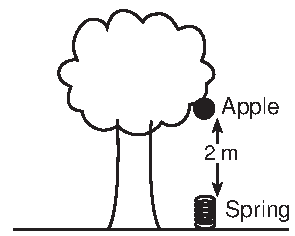
\includegraphics[keepaspectratio]{Jan2004-Q16}
    \end{center}
    The apple falls and hits the spring compressing it \SI{0.1}{\meter} from its rest position.
    If all of the gravitational potential energy of the apple on the tree is transferred to the spring when it is compressed,
        what is the spring constant of the spring?
    \begin{multicols}{2}
    \begin{choices}
      \correctchoice{\SI{400}{\newton\per\meter}}
        \wrongchoice{\SI{10}{\newton\per\meter}}
        \wrongchoice{\SI{100}{\newton\per\meter}}
        \wrongchoice{\SI{40}{\newton\per\meter}}
    \end{choices}
    \end{multicols}
\end{question}
}

\element{nysed}{
\begin{question}{Jan2004-Q17}
    A \SI{1}{\kilo\gram} rock is dropped from a cliff \SI{90}{\meter} high.
    After falling \SI{20}{\meter},
        the kinetic energy of the rock is approximately:
    \begin{multicols}{2}
    \begin{choices}
      \correctchoice{\SI{200}{\joule}}
        \wrongchoice{\SI{20}{\joule}}
        \wrongchoice{\SI{700}{\joule}}
        \wrongchoice{\SI{900}{\joule}}
    \end{choices}
    \end{multicols}
\end{question}
}


%% Section June2003
%%--------------------
\element{nysed}{
\begin{question}{June2003-Q18}
    As a ball falls freely (without friction) toward the ground,
        its total mechanical energy:
    \begin{choices}
      \correctchoice{remains the same}
        \wrongchoice{decreases}
        \wrongchoice{increases}
    \end{choices}
\end{question}
}

\element{nysed}{
\begin{question}{June2003-Q19}
    A \SI{0.50}{\kilo\gram} ball is thrown vertically upward with an initial kinetic energy of \SI{25}{\joule}.
    Approximately how high will the ball rise?
    [Neglect air resistance.]
    \begin{multicols}{2}
    \begin{choices}
      \correctchoice{\SI{5.1}{\meter}}
        \wrongchoice{\SI{2.6}{\meter}}
        \wrongchoice{\SI{13}{\meter}}
        \wrongchoice{\SI{25}{\meter}}
    \end{choices}
    \end{multicols}
\end{question}
}

\element{nysed}{
\begin{question}{June2003-Q42}
    Which graph best represents the relationship between kinetic energy and the velocity of an object accelerating in a straight line?
    \begin{multicols}{2}
    \begin{choices}
        \AMCboxDimensions{down=-2.5em}
        \correctchoice{
            \begin{tikzpicture}
                \begin{axis}[
                    axis y line=left,
                    axis x line=bottom,
                    axis line style={->},
                    xlabel={velocity},
                    xtick=\empty,
                    ylabel={kinetic energy},
                    ytick=\empty,
                    xmin=0,xmax=11,
                    ymin=0,ymax=11,
                    width=\columnwidth,
                    very thin,
                ]
                \addplot[line width=1pt,domain=0:10]{7};
                \end{axis}
            \end{tikzpicture}
        }
        \wrongchoice{
            \begin{tikzpicture}
                \begin{axis}[
                    axis y line=left,
                    axis x line=bottom,
                    axis line style={->},
                    xlabel={velocity},
                    xtick=\empty,
                    ylabel={kinetic energy},
                    ytick=\empty,
                    xmin=0,xmax=11,
                    ymin=0,ymax=11,
                    width=\columnwidth,
                    very thin,
                ]
                \addplot[line width=1pt,domain=0:10]{x};
                \end{axis}
            \end{tikzpicture}
        }
        \wrongchoice{
            \begin{tikzpicture}
                \begin{axis}[
                    axis y line=left,
                    axis x line=bottom,
                    axis line style={->},
                    xlabel={velocity},
                    xtick=\empty,
                    ylabel={kinetic energy},
                    ytick=\empty,
                    xmin=0,xmax=11,
                    ymin=0,ymax=11,
                    width=\columnwidth,
                    very thin,
                ]
                \addplot[line width=1pt,domain=0:10]{5/x};
                \end{axis}
            \end{tikzpicture}
        }
        \wrongchoice{
            \begin{tikzpicture}
                \begin{axis}[
                    axis y line=left,
                    axis x line=bottom,
                    axis line style={->},
                    xlabel={velocity},
                    xtick=\empty,
                    ylabel={kinetic energy},
                    ytick=\empty,
                    xmin=0,xmax=11,
                    ymin=0,ymax=11,
                    width=\columnwidth,
                    very thin,
                ]
                \addplot[line width=1pt,domain=0:10]{0.1*x*x};
                \end{axis}
            \end{tikzpicture}
        }
    \end{choices}
    \end{multicols}
\end{question}
}


%% Section Jan2003
%%--------------------
\element{nysed}{
\begin{question}{Jan2003-Q16}
    As an object falls freely,
        the kinetic energy of the object:
    \begin{choices}
      \correctchoice{increases}
        \wrongchoice{decreases}
        \wrongchoice{remains the same}
    \end{choices}
\end{question}
}

\element{nysed}{
\begin{question}{Jan2003-Q39}
    A constant force is used to keep a block sliding at constant velocity along a rough horizontal track.
    As the block slides, there could be an increase in its:
    \begin{choices}
      \correctchoice{internal energy, only}
        \wrongchoice{gravitational potential energy, only}
        \wrongchoice{gravitational potential energy and kinetic energy}
        \wrongchoice{internal energy and kinetic energy}
    \end{choices}
\end{question}
}


%% Section June2002
%%--------------------
\element{nysed}{
\begin{question}{Jan2002-Q16}
    What is an essential characteristic of an object in equilibrium?
    \begin{choices}
        \wrongchoice{zero velocity}
      \correctchoice{zero acceleration}
        \wrongchoice{zero potential energy}
        \wrongchoice{zero kinetic energy}
    \end{choices}
\end{question}
}

\element{nysed}{
\begin{question}{June2002-Q43}
    Which graph best represents the relationship between the gravitational potential energy of a freely falling object and the object's height above the ground near the surface of Earth.
    \begin{multicols}{2}
    \begin{choices}
        \AMCboxDimensions{down=-2.5em}
        \wrongchoice{
            \begin{tikzpicture}
                \begin{axis}[
                    axis y line=left,
                    axis x line=bottom,
                    axis line style={->},
                    xlabel={height},
                    xtick=\empty,
                    ylabel={energy},
                    ytick=\empty,
                    xmin=0,xmax=11,
                    ymin=0,ymax=11,
                    width=\columnwidth,
                    very thin,
                ]
                \addplot[line width=1pt,domain=0:10]{x};
                \end{axis}
            \end{tikzpicture}
        }
        \correctchoice{
            \begin{tikzpicture}
                \begin{axis}[
                    axis y line=left,
                    axis x line=bottom,
                    axis line style={->},
                    xlabel={height},
                    xtick=\empty,
                    ylabel={energy},
                    ytick=\empty,
                    xmin=0,xmax=11,
                    ymin=0,ymax=11,
                    width=\columnwidth,
                    very thin,
                ]
                \addplot[line width=1pt,domain=0:10]{10-x};
                \end{axis}
            \end{tikzpicture}
        }
        \wrongchoice{
            \begin{tikzpicture}
                \begin{axis}[
                    axis y line=left,
                    axis x line=bottom,
                    axis line style={->},
                    xlabel={height},
                    xtick=\empty,
                    ylabel={energy},
                    ytick=\empty,
                    xmin=0,xmax=11,
                    ymin=0,ymax=11,
                    width=\columnwidth,
                    very thin,
                ]
                \addplot[line width=1pt,domain=0:10]{8};
                \end{axis}
            \end{tikzpicture}
        }
        \wrongchoice{
            \begin{tikzpicture}
                \begin{axis}[
                    axis y line=left,
                    axis x line=bottom,
                    axis line style={->},
                    xlabel={height},
                    xtick=\empty,
                    ylabel={energy},
                    ytick=\empty,
                    xmin=0,xmax=11,
                    ymin=0,ymax=11,
                    width=\columnwidth,
                    very thin,
                ]
                \addplot[line width=1pt,domain=0:10]{0.1*x*x};
                \end{axis}
            \end{tikzpicture}
        }
    \end{choices}
    \end{multicols}
\end{question}
}


%% Section June1998
%%--------------------
\element{nysed}{
\begin{question}{June1998-Q19}
    The diagram below shows a \SI{1.5}{\kilo\gram} kitten jumping from the top of a \SI{1.80}{\meter} high refrigerator to a \SI{0.90}{\meter} high counter.
    \begin{center}
        %% NOTE: keep graphic
        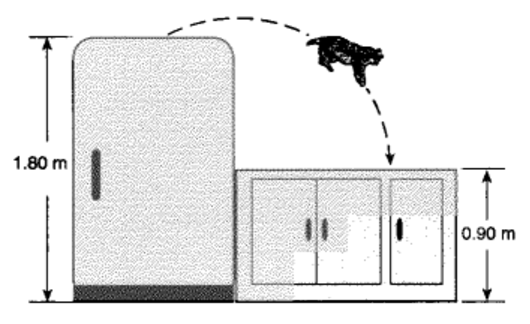
\includegraphics[keepaspectratio,scale=0.95]{June1998-Q19}
    \end{center}
    Compared to the kitten's gravitational potential energy on top of the refrigerator,
        the kitten's gravitational potential energy on top of the counter is:
    \begin{choices}
      \correctchoice{half as great}
        \wrongchoice{twice as great}
        \wrongchoice{one-fourth as great}
        \wrongchoice{four times as great}
    \end{choices}
\end{question}
}


%% Section June1997
%%--------------------


%% Section June1994
%%--------------------
\element{nysed}{
\begin{question}{June1994-Q22}
    In the diagram below, an ideal pendulum released from point $A$ swings freely through point $B$.
    \begin{center}
    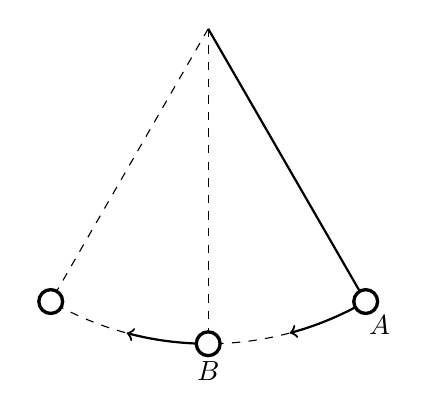
\begin{tikzpicture}
        %% strings
        \draw[thick] (0,0) -- (300:4);
        \draw[dashed] (0,0) -- (270:4);
        \draw[dashed] (0,0) -- (240:4);
        %% path
        \draw[dashed] (300:4) arc (300:240:4);
        \draw[thick,->] (300:4) arc (300:285:4);
        \draw[thick,->] (270:4) arc (270:255:4);
        %% options
        \foreach \x/\y in {300/A,270/B,240/} {
            \draw[very thick,fill=white] (\x:4) circle (1ex);
            \node[anchor=center,shift={(\x:1em)}] at (\x:4) {$\y$};
        }
    \end{tikzpicture}
    \end{center}
    Compared to the pendulum's kinetic energy at $A$,
        its potential energy at $B$ is:
    \begin{multicols}{2}
    \begin{choices}
        \wrongchoice{half as great}
        \wrongchoice{twice as great}
      \correctchoice{the same}
        \wrongchoice{four times as great}
    \end{choices}
    \end{multicols}
\end{question}
}


\endinput


